\section{Alloy}
\lstset{
  language=alloy,
  basicstyle=\small\ttfamily,
  breaklines=true,
  showstringspaces=false
}
\lstinputlisting{4Alloy/res/third_model.als}

In this section it is provided a representation of the world of CKB using the Alloy language. Every run and every check are commented in order to guarantee a syntactical correct compilation of the code: it is up to the reader to decide what to uncomment based on their will.

\subsection{Generated World}
\begin{figure}[h]
  \centering
  %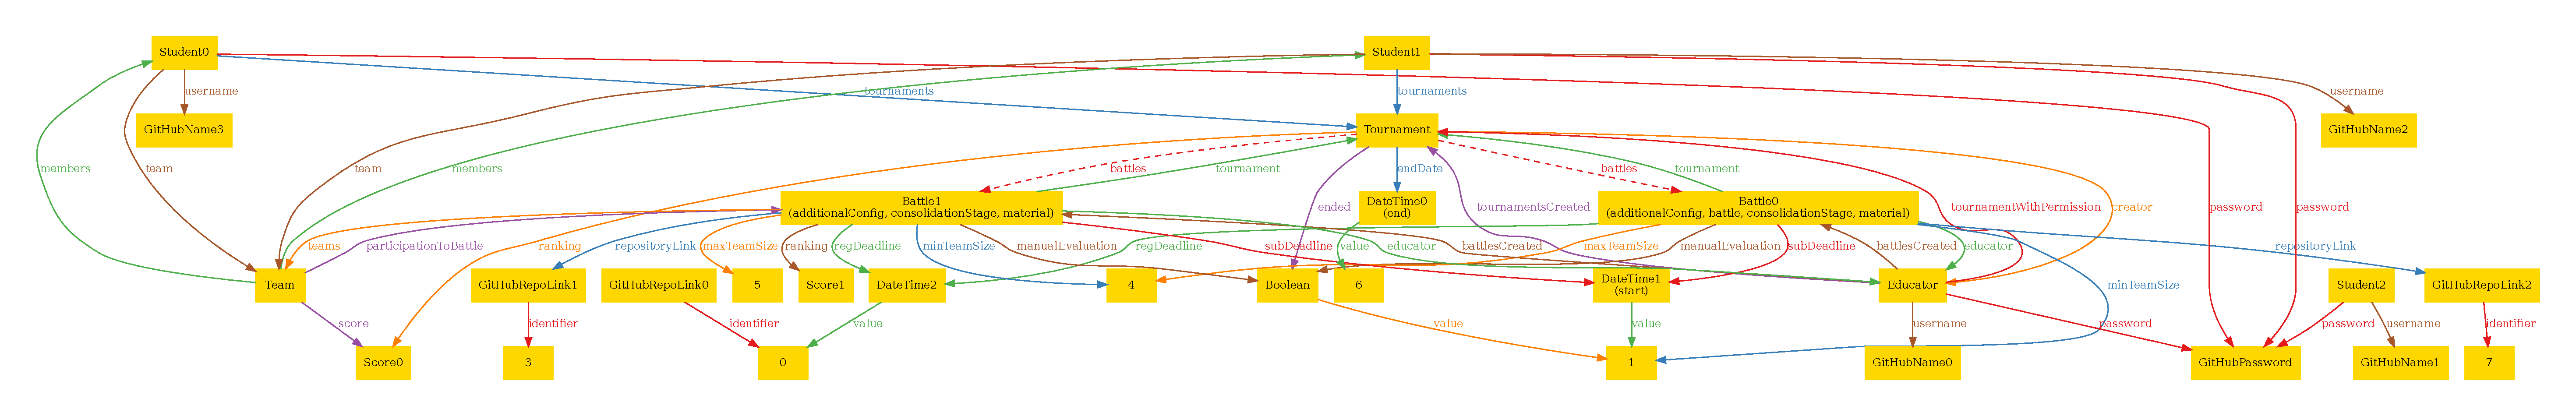
\includegraphics[width=1\linewidth]{RASD/4Alloy/res/general.pdf}
  \caption{The world generated by running \textit{general} projected over nine signatures (ABS, Boolean, CodeTest, DateTime, GitHubName, Int, Macrovariables, Password, SourceCode) in order to be more comprehensible}
\end{figure}

\begin{figure}[h]
  \centering
  %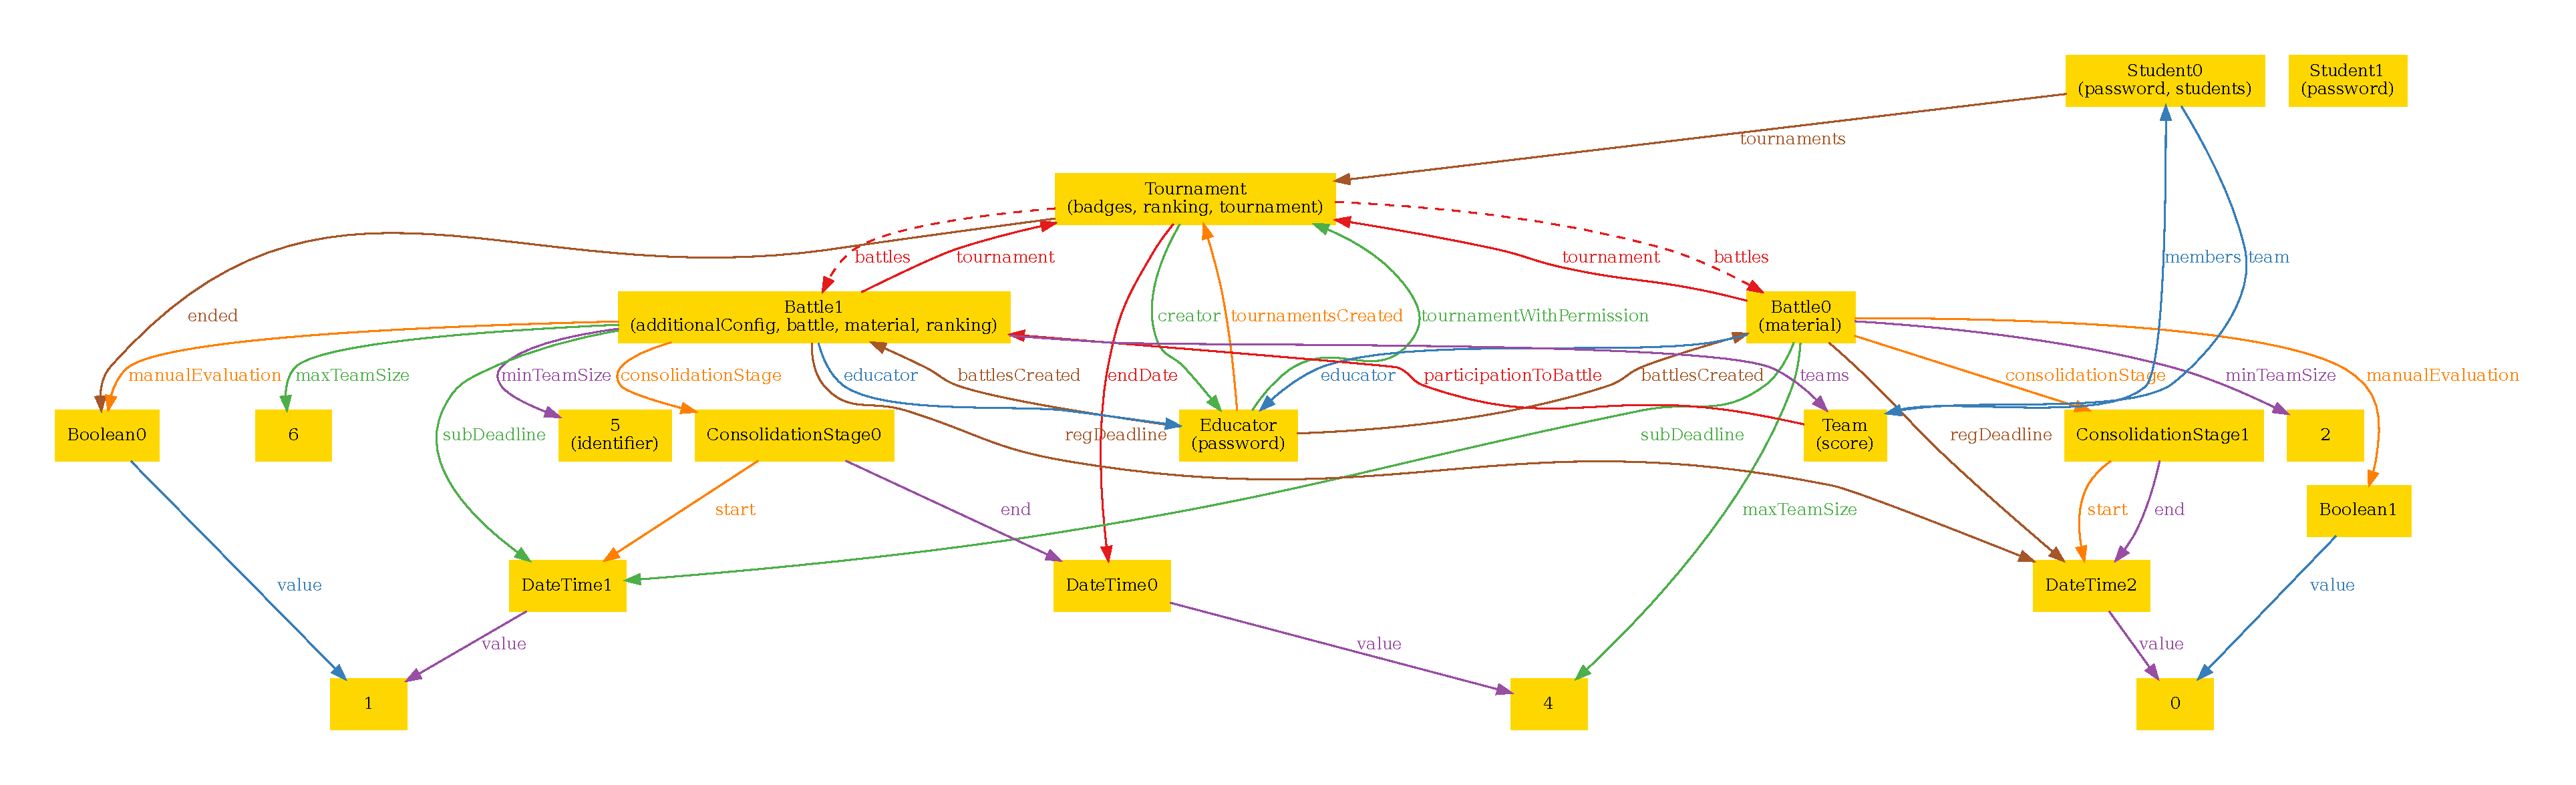
\includegraphics[width=1\linewidth]{RASD/4Alloy/res/noManualEvaluation.pdf}
  \caption{The world generated by running \textit{noManualEvaluation} projected over eleven signatures (ABS, Badge, Code, CodeTest, DateTime, GitHubName, GitHubRepoLink, Macrovariables, Password, SourceCode, String) in order to be more comprehensible. This world exploit the situation where there is no manual evaluation for one battle out of two. It is useful in order to see the right aim of the model. Indeed, as you can see, in the case the manualEvaluation is not required (boolean value of 0) there is no consolidation stage, and viceversa}
\end{figure}

The representation of the world at the instant 1 is here omitted due to the fact it only modifies one of the value among the signatures.
